Στο κεφάλαιο αυτό παρουσιάζεται αναλυτικά η μελέτη της δυναμικής συμπεριφοράς ενός διακριτού συστήματος που αποτελεί παραλλαγή του γνωστού Χάρτη Chebysev. Για επιλεγμένες τιμές της παραμέτρου του μπορεί να παρουσιάσει χαοτική συμπεριφορά όπως και φαινόμενα που σχετίζονται με τη μη-γραμμική δυναμική. Για τη μελέτη χρησιμοποιήθηκαν τα διαγράμματα διακλάδωσης, οι εκθέτες Lyapunov και οι απεικονίσεις της τιμής \(x_i\) σε συνάρτηση με  την τιμή \(x_{i+1}\).

Ο Χάρτης Chebysev  που αποτέλεσε τη βάση του προτεινόμενου σε αυτή την ενότητα, χάρτη, περιγράφεται από την παρακάτω εξίσωση \cite{b9}:

\begin{equation}
	x_{i+1}=\cos(k*\arccos(x_i))
	\label{f:x4}
\end{equation}


Στην εξίσωση (\ref{f:x4}) χρησιμοποιήθηκε ένας σταθερός όρος q. Έτσι προέκυψε η προτεινόμενη παραλλαγή του Χάρτη Chebysev,

\begin{equation}
	x_{i+1}=\cos(k^q\arccos(q*x_i))
	\label{f:x5}
\end{equation}
όπου k, q παράμετροι.\\

Για την εύρεση της δυναμικής συμπεριφοράς του συστήματος εξετάστηκε μια περιοχή τιμών των παραμέτρων του. Πιο συγκεκριμένα, στη μελέτη που πραγματοποιήθηκε η αρχική συνθήκη του $x_0 =0.1$ παρέμεινε  σταθερή, ενώ η τιμή της παραμέτρου q μεταβαλλόταν στο διάστημα $[0.8,0.9]$ με βήμα $0.1$. Έτσι, για κάθε περίπτωση παράχθηκαν το διάγραμμα διακλάδωσης, το διάγραμμα των εκθετών Lyapunov και το διάγραμμα της τιμής \(x_i\) σε συνάρτηση με  την τιμή \(x_{i+1}\), τα οποία παρουσιάζονται και αναλύονται στη συνέχεια.\\

\vspace{\fill}


\section{Για \emph{q} = 0.8}

Στo Σχ. \ref{f:g59} παρατίθεται τα διάγραμμα διακλάδωσης του συστήματος του Σχ. \ref{f:x5}, ως προς τη παράμετρο k, για $q =0.8$. Στον Πίνακα \ref{tab:abc12} φαίνεται η πορεία του συστήματος και για ποιες τιμές της παραμέτρου k το σύστημα εμφανίζει περιοδική ή χαοτική συμπεριφορά, σύμφωνα με το διάγραμμα διακλάδωσης του Σχ. \ref{f:g44}. Επίσης παρατηρείται συνοριακή κρίση ελκυστών για διάφορες τιμές του k (2.65, 2.938, 3.147, 3.45, 3.642, 3.776, 3.886, 4.1, 4.155), όπως και το φαινόμενο της εσωτερικής κρίσης το οποίο φαίνεται στο διάγραμμα διακλάδωσης του Σχ. \ref{f:g63}. Οι αντίστοιχες τιμές του k για αυτά τα σημεία του διαγράμματος υπάρχουν στον Πίνακα \ref{tab:abc12}, όπως και τα αντίστοιχα διαγράμματα της τιμής \(x_i\) σε συνάρτηση με την τιμή \(x_{i+1}\) στο Σχ. \ref{f:k249} . Από τα παραγόμενα σχήματα προκύπτει αριθμός σημείων αντίστοιχος με την περίοδο του συστήματος.

Επιπλέον παρατηρούμε στo Σχ. \ref{f:g64}, το φαινόμενο της αντιμονοτονικότητας. Στα τρία διαγράμματα του Σχ. \ref{f:g64} εμφανίζονται τρεις διαφορετικές περιπτώσεις του φαινομένου αυτού. Ενώ παρατηρούνται χαοτικές φυσαλίδες (το σύστημα εισέρχεται στο χάος με διπλασιασμό της περιόδου και στην συνέχεια εξέρχεται από αυτό με υποδιπλασιασμό της περιόδου) σε όλες τις περιπτώσεις , η αρχική περίοδος είναι διαφορετική για κάθε περιοχή(\ref{f:g61} - \emph(περίοδος - 5), \ref{f:g62} - \emph(περίοδος - 4), \ref{f:g63} - \emph(περίοδος - 2)). 

Τέλος, στο σχήμα \ref{f:g60} παρατίθεται το διάγραμμα των εκθετών Lyapunov για τιμές του k στο ίδιο διάστημα τιμών $[0, 4.4]$. Οι τιμές του Πίνακα \ref{tab:abc12} που έχουν περιοδική συμπεριφορά αντιστοιχούν σε τιμές του διαγράμματος του Σχ. \ref{f:g59}, όπου o εκθέτης Lyapunov είναι συνεχώς αρνητικός, γεγονός που επιβεβαιώνει την συμπεριφορά του. Για τις υπόλοιπες τιμές ο θετικός εκθέτης Lyapunov υποστηρίζει την χαοτική του συμπεριφορά, όπως γίνεται φανερό και από το διάγραμμα διακλάδωσης.\\\\

\begin{table}[ht]
	\centering
	\caption{ Συμπεριφορά του υπό μελέτη συστήματος για διάφορες τιμές του k, για $q=0.8$. }
	\label{tab:abc12}
	\begin{tabular}{l | l}
		Παράμετρος k & Συμπεριφορά \\
		\hline
		1.3 &  Περίοδος -  1 \\
		1.86 &  Περίοδος -  2 \\
		2.34& Περίοδος -  4 \\
		2.49& Περίοδος -  8 \\
		2.52& Περίοδος -  16 \\
		2.53 & Xάος \\
		2.65& Περίοδος - 6 \\
		2.655& Περίοδος - 12\\
		2.66& Χάος \\
		2.938& Περίοδος - 5 \\
		2.95 &  Περίοδος - 10  \\
		2.971 &  Περίοδος -  20 \\
		2.975 &  Χάος \\
		3.147& Περίοδος - 20 \\
		3.15 &  Περίοδος - 10  \\
		3.17 &  Περίοδος -  5 \\
		3.24 &Περίοδος - 10 \\
		3.258 &  Περίοδος -  5\\
		3.28 &Χάος \\
		3.45 & Περίοδος - 4\\
		3.453& Περίοδος - 8\\
		3.455& Περίοδος - 16\\
		3.46& Xάος\\
		3.642& Περίοδος - 16\\
		3.643 & Περίοδος - 8\\
		3.647& Περίοδος - 4\\
		3.65 & Χάος\\
		3.776 & Περίοδος -  2\\
		3.82 & Περίοδος -  4\\
		3.85 & Περίοδος -  8\\
		3.86 & Xάος\\
		3.886 & Περίοδος -  6\\
		3.887 & Περίοδος -  12\\
		3.888 & Χάος\\
		4.1& Περίοδος -  24\\
		4.101& Περίοδος -  12\\
		4.102 & Περίοδος -  6\\
		4.108 & Χάος\\
		4.155 & Περίοδος -  8\\
		4.17 & Περίοδος -  4\\
		4.22 & Περίοδος -  2\\
		4.32 &  Χάος\\
		
	\end{tabular}
	
\end{table}

\begin{figure}[ht]
	\centering
	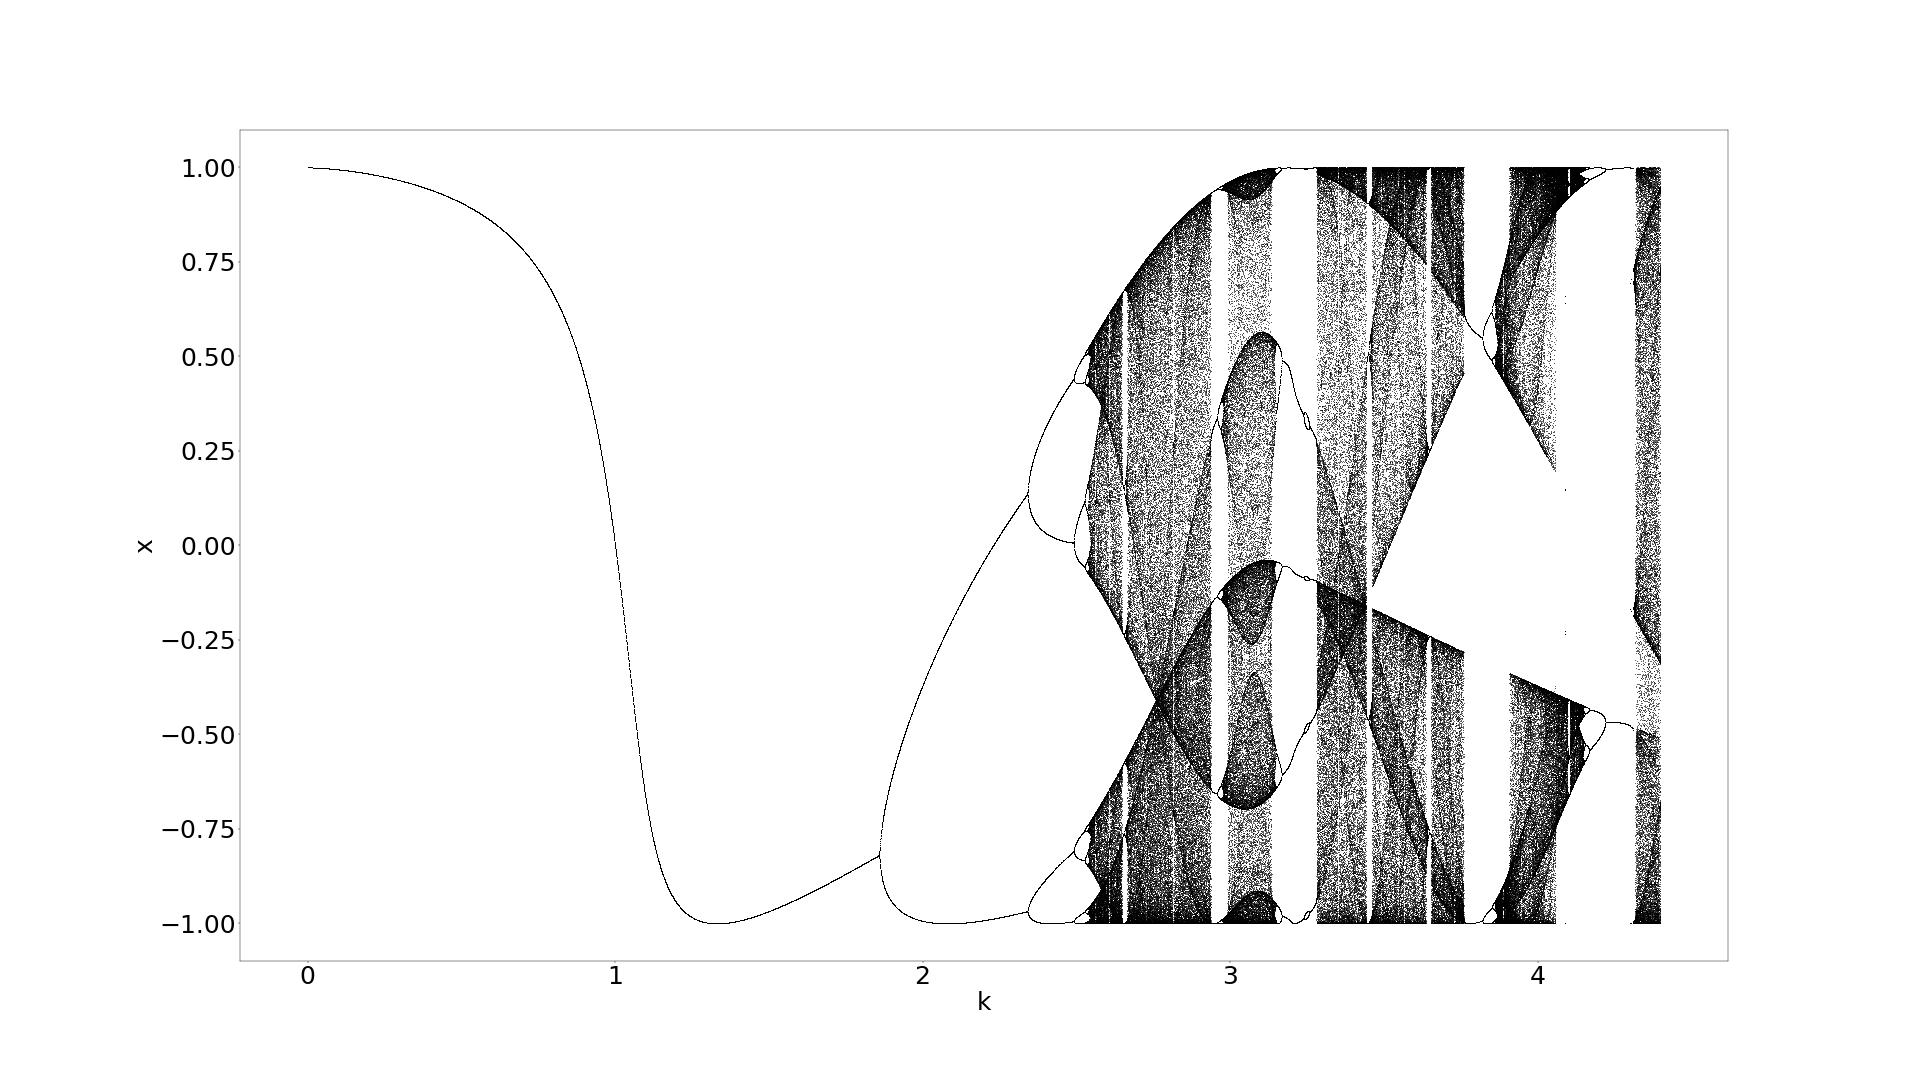
\includegraphics[width=1\linewidth]{LateX images/cheb q=0.8/g1}
	\caption{Διάγραμμα διακλάδωσης, για $q=0.8$.}
	\label{f:g59}
\end{figure}


\begin{figure}[ht]
	\centering
	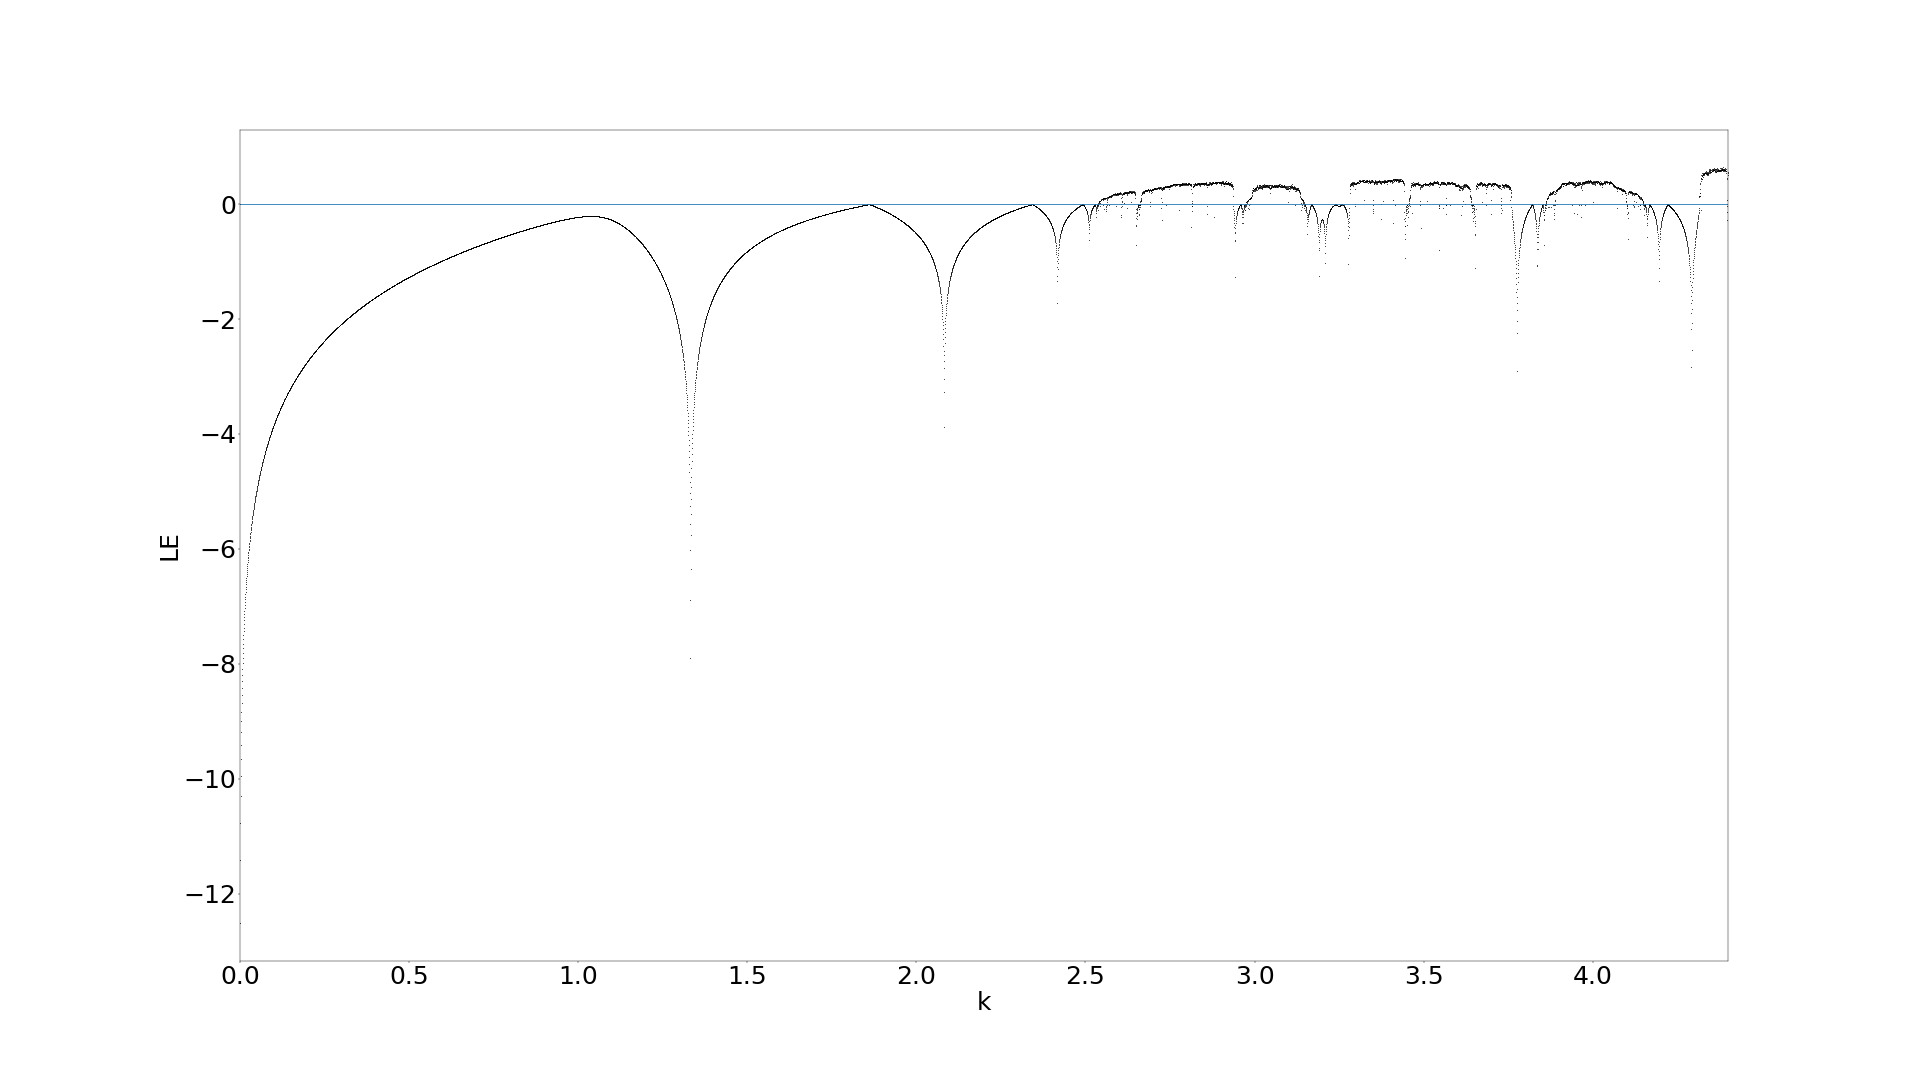
\includegraphics[width=1\linewidth]{LateX images/cheb q=0.8/g2}
	\caption{Διάγραμμα των εκθετών Lyapunov σε συνάρτηση με την παράμετρο k, για $q=0.8$.}
	\label{f:g60}
\end{figure}


\begin{figure}[ht]
	\centering
	
	\begin{subfigure}[b]{0.8\textwidth}
		\centering
		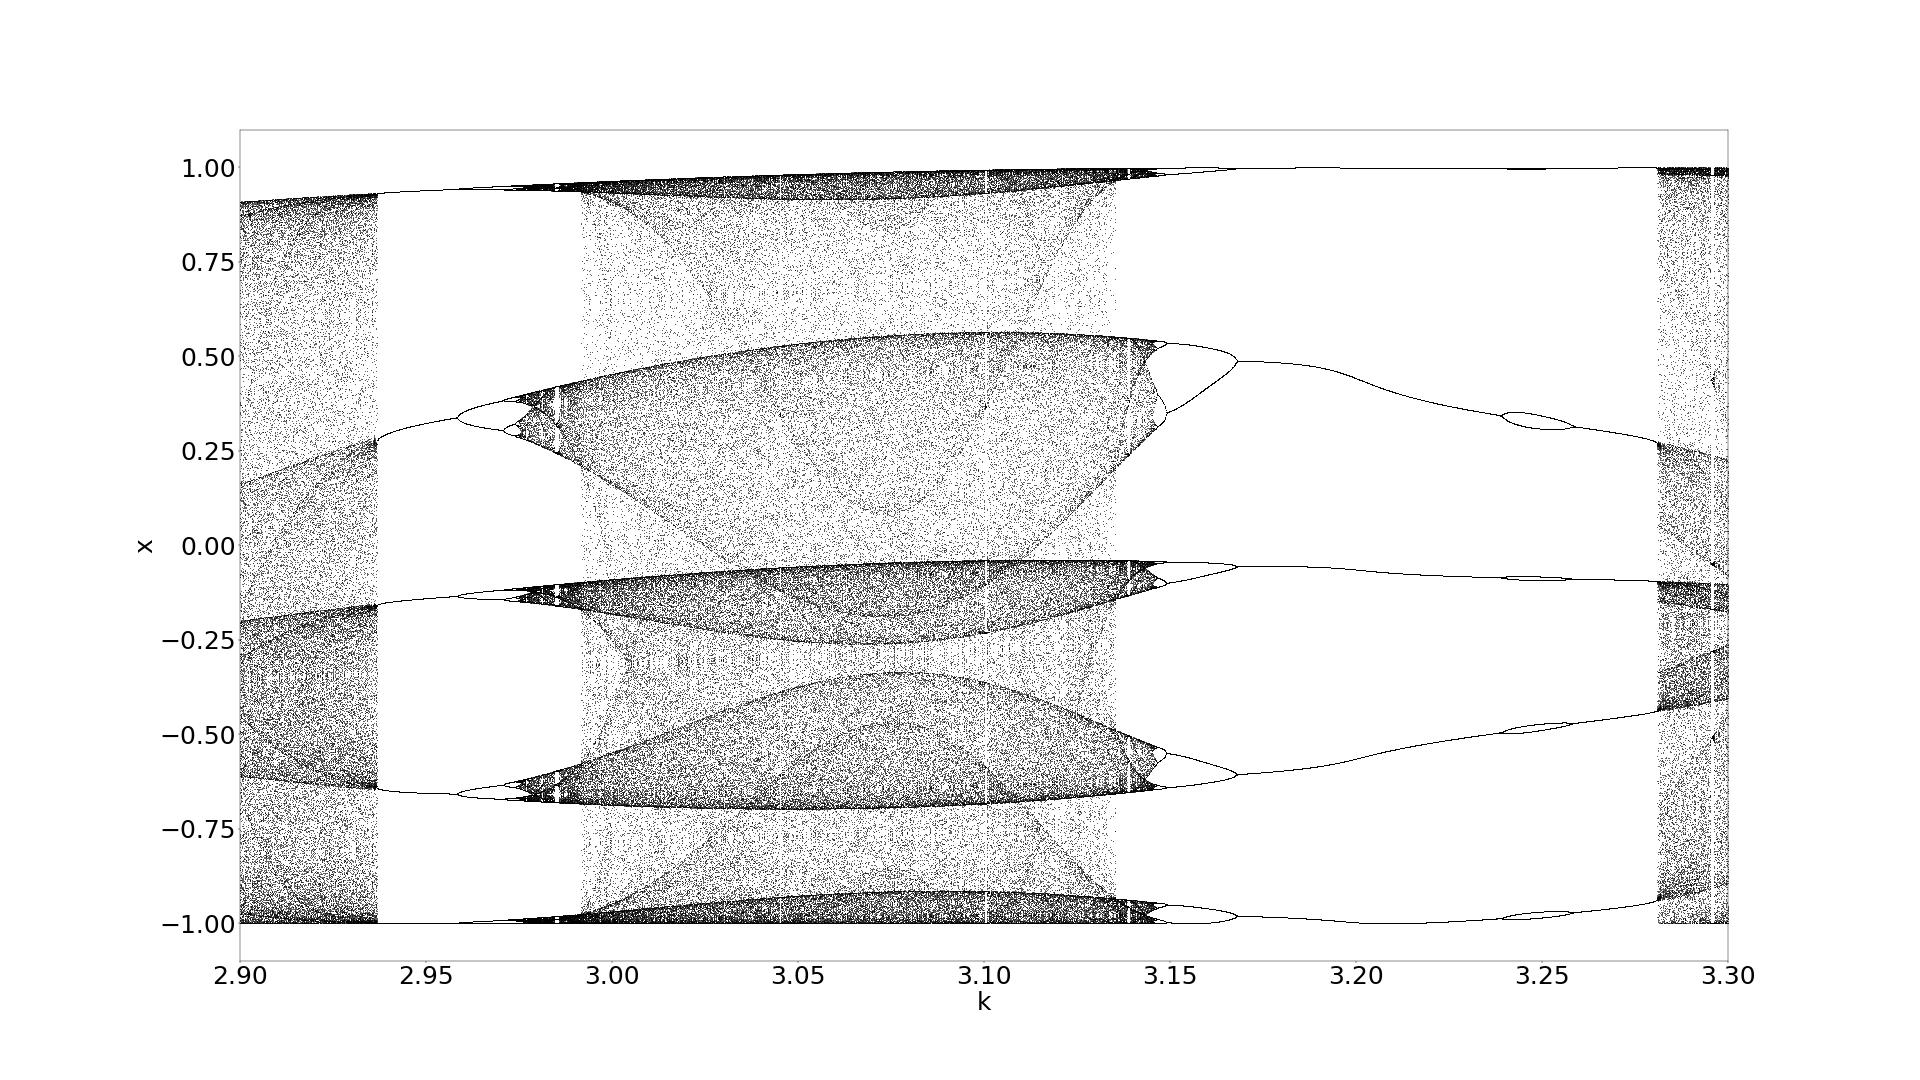
\includegraphics[width=\textwidth]{LateX images/cheb q=0.8/g3}
		\caption{Για $2.9<k<3.3$}
		\label{f:g61}
	\end{subfigure}
	\hfill
	\begin{subfigure}[b]{0.8\textwidth}
		\centering
		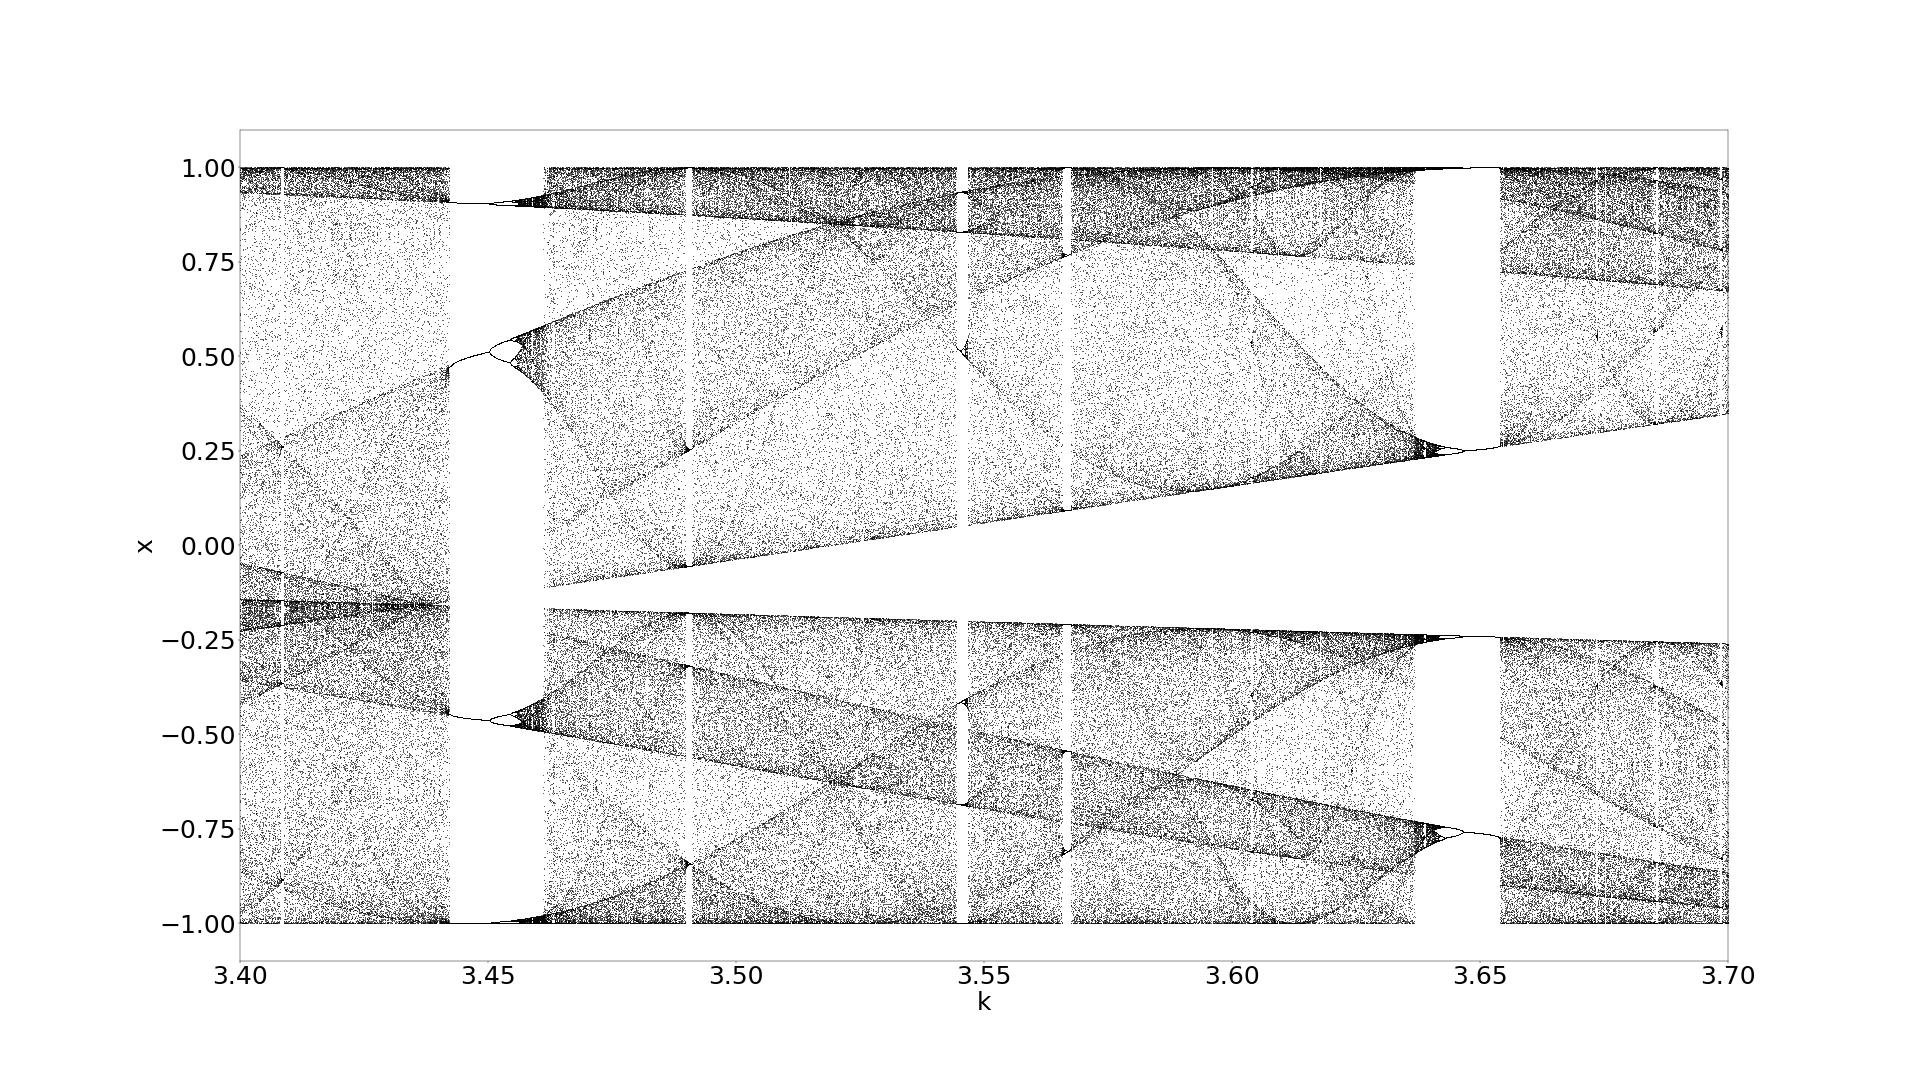
\includegraphics[width=\textwidth]{LateX images/cheb q=0.8/g4}
		\caption{Για $3.4<k<3.7$}
		\label{f:g62}
	\end{subfigure}
	\hfill
	\begin{subfigure}[b]{0.8\textwidth}
		\centering
		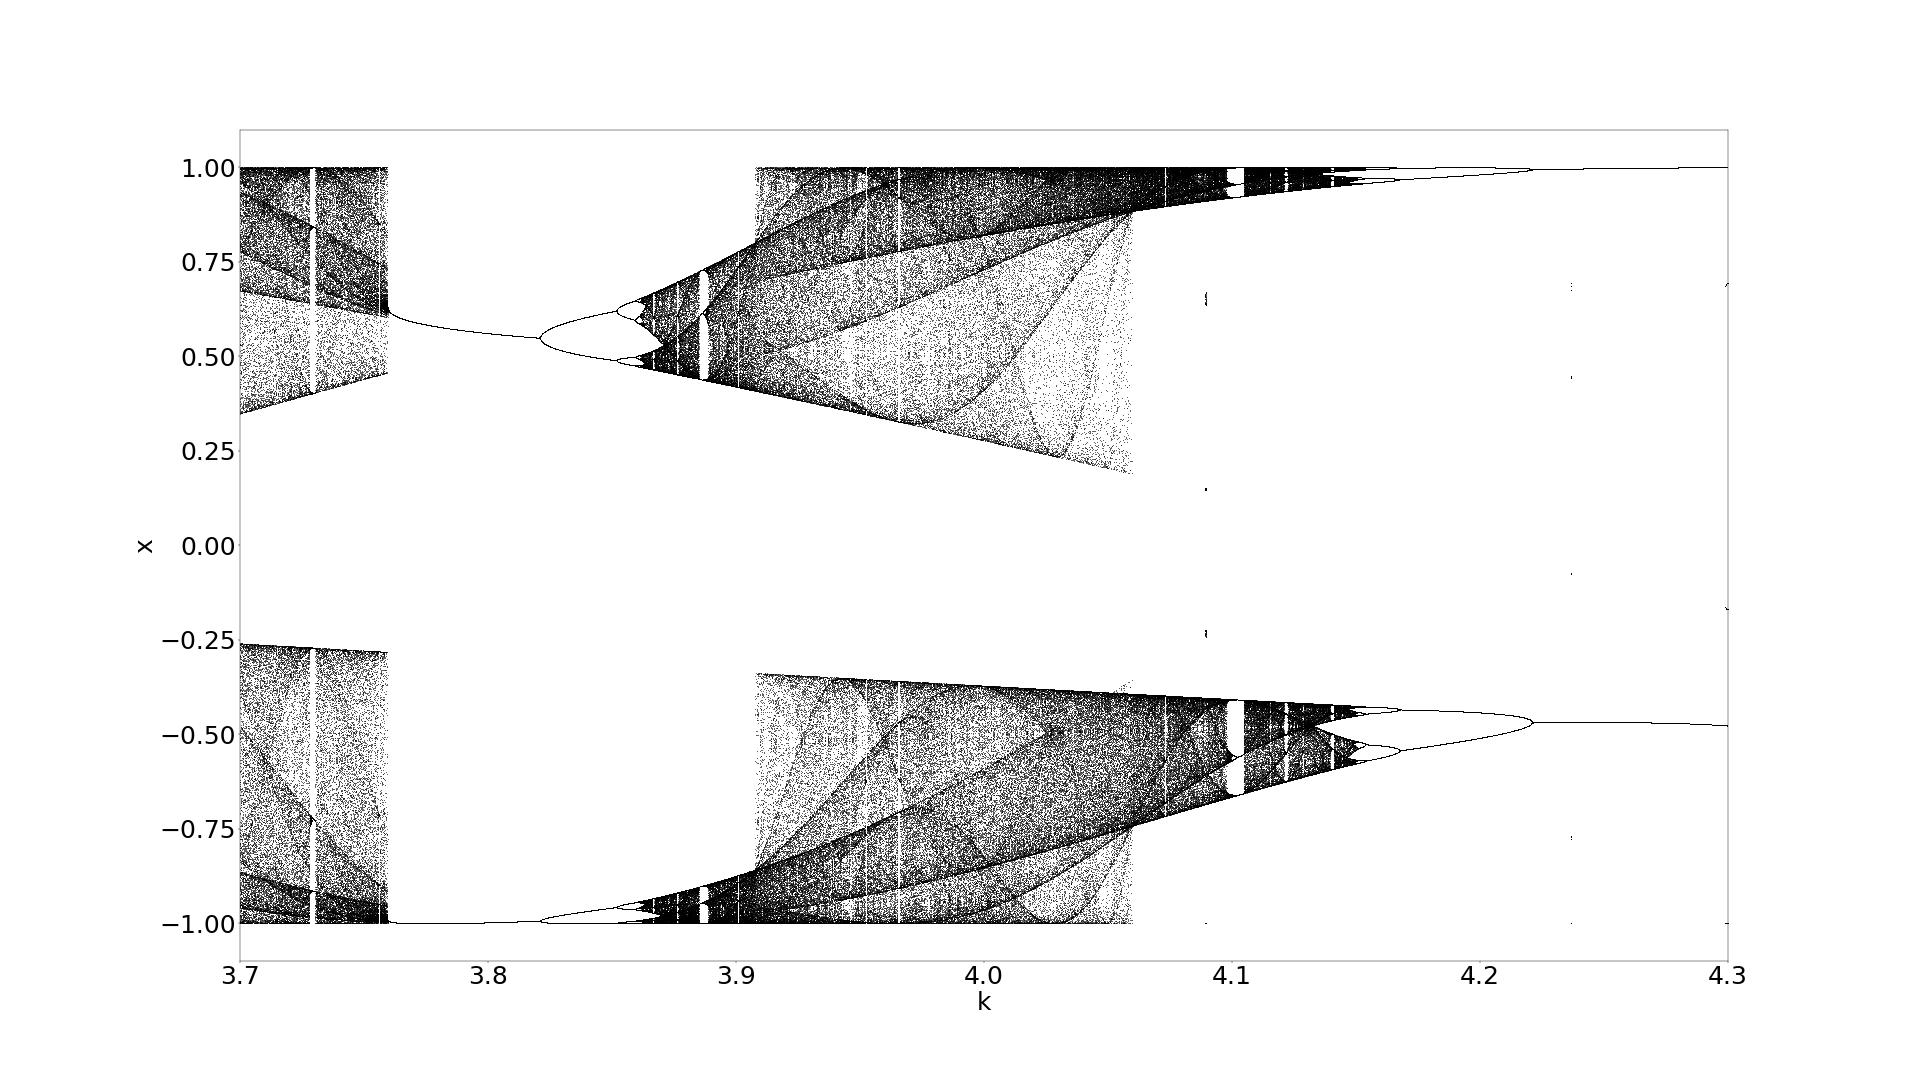
\includegraphics[width=\textwidth]{LateX images/cheb q=0.8/g5}
		\caption{Για $3.6<k<4.7$}
		\label{f:g63}
	\end{subfigure}
	
	\caption{Διαγράμματα διακλάδωσης για διάφορες τιμές του $k$. }
	\label{f:g64}
\end{figure}

\begin{figure}[ht]
	\centering
	\begin{subfigure}[b]{0.4\textwidth}
		\centering
		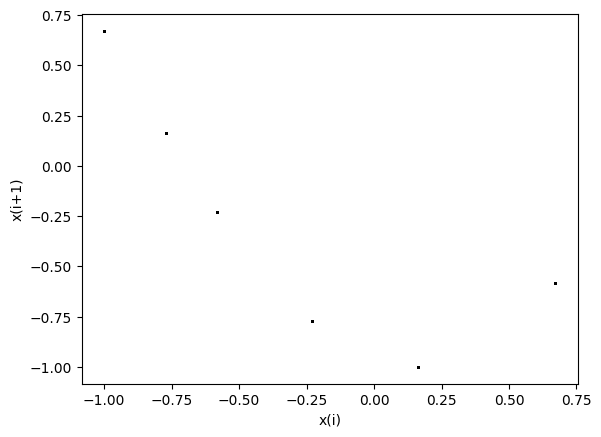
\includegraphics[width=\textwidth]{LateX images/cheb q=0.8/g6}
		\caption{Για $k=2.65$}
		\label{f:k133}
	\end{subfigure}
	\hfill
	\begin{subfigure}[b]{0.4\textwidth}
		\centering
		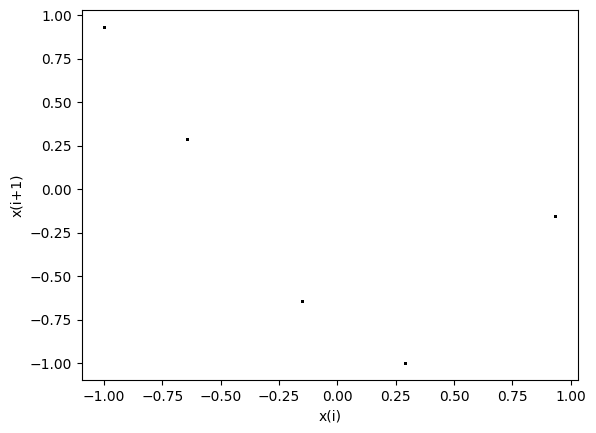
\includegraphics[width=\textwidth]{LateX images/cheb q=0.8/g7}
		\caption{Για $k=2.938$}
		\label{f:k134}
	\end{subfigure}
	\hfill
	\begin{subfigure}[b]{0.4\textwidth}
		\centering
		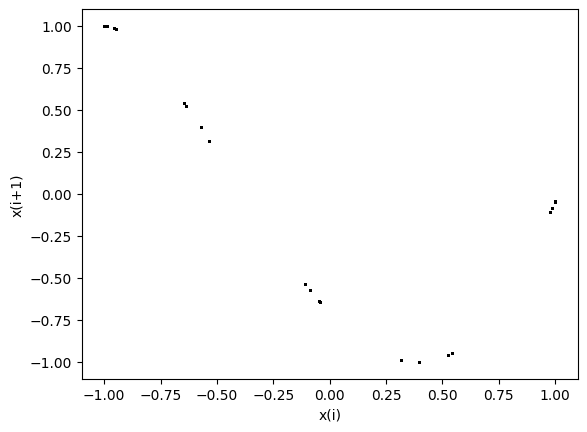
\includegraphics[width=\textwidth]{LateX images/cheb q=0.8/g8}
		\caption{Για $k=3.147$}
		\label{f:k135}
	\end{subfigure}
	\hfill
	\begin{subfigure}[b]{0.4\textwidth}
		\centering
		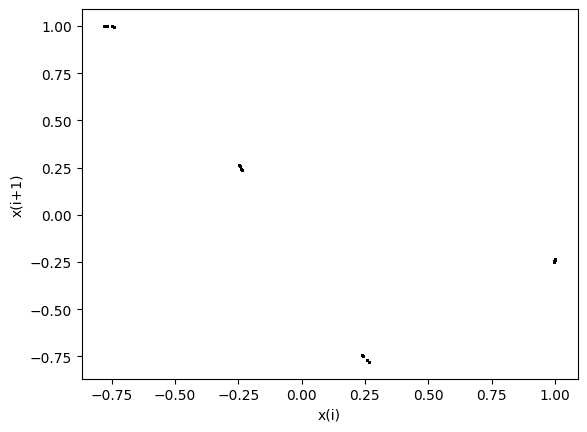
\includegraphics[width=\textwidth]{LateX images/cheb q=0.8/g10}
		\caption{Για $k=3.642$}
		\label{f:k137}
	\end{subfigure}
	\hfill	
	\begin{subfigure}[b]{0.4\textwidth}
		\centering
		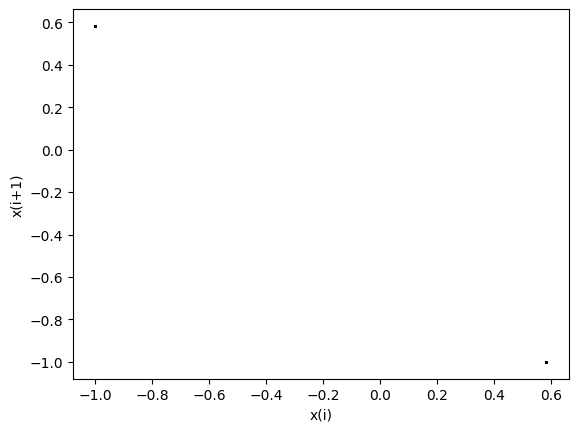
\includegraphics[width=\textwidth]{LateX images/cheb q=0.8/g11}
		\caption{Για $k=3.776$}
		\label{f:k138}
	\end{subfigure}
	\hfill
	\begin{subfigure}[b]{0.4\textwidth}
		\centering
		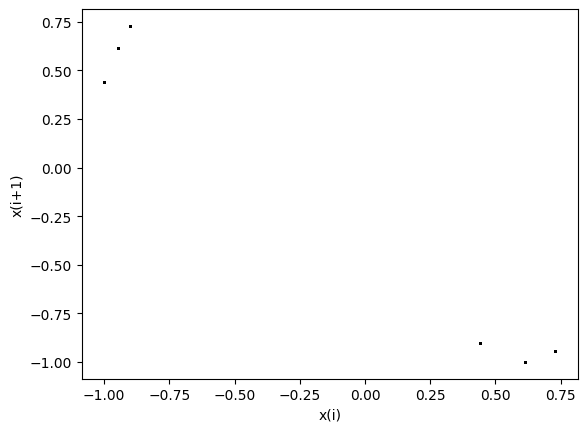
\includegraphics[width=\textwidth]{LateX images/cheb q=0.8/g12}
		\caption{Για $k=3.886$}
		\label{f:k139}
	\end{subfigure}
	\hfill
	\begin{subfigure}[b]{0.4\textwidth}
		\centering
		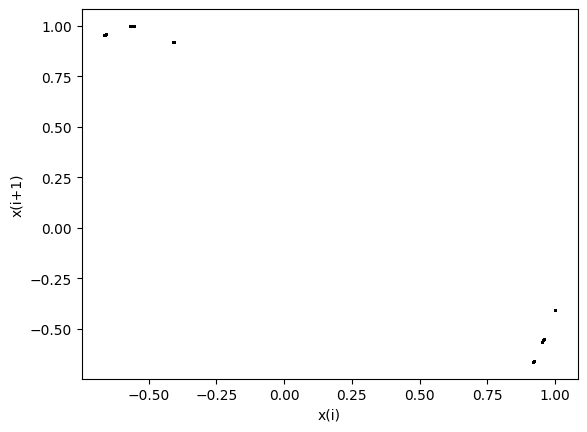
\includegraphics[width=\textwidth]{LateX images/cheb q=0.8/g13}
		\caption{Για $k=4.1$}
		\label{f:k140}
	\end{subfigure}
	\hfill
	\begin{subfigure}[b]{0.4\textwidth}
		\centering
		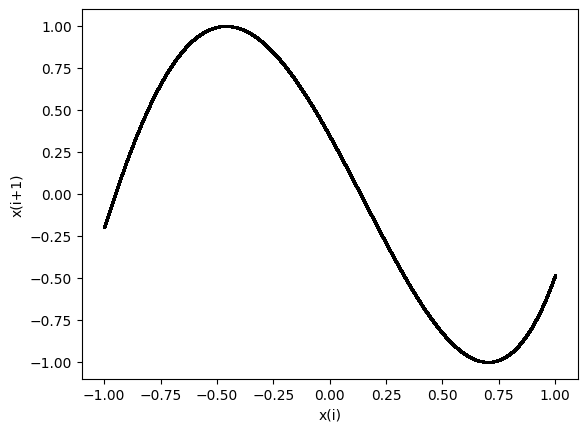
\includegraphics[width=\textwidth]{LateX images/cheb q=0.8/g9}
		\caption{Για $k=4.32$}
		\label{f:k136}
	\end{subfigure}
	\hfill	
	\caption{Διαγράμματα της τιμής \(x_i\) σε συνάρτηση με την τιμή \(x_{i+1}\).}
	\label{f:k249}
\end{figure}

\clearpage

\section{Για \emph{q} = 0.9}

Στo Σχ. \ref{f:g65} παρατίθεται τα διάγραμμα διακλάδωσης του συστήματος (\ref{f:x5}), ως προς την παράμετρο k, για $q =0.9$. Στον Πίνακα \ref{tab:abc13} φαίνεται η πορεία του συστήματος και για ποιες τιμές της παραμέτρου k το σύστημα εμφανίζει περιοδική ή χαοτική συμπεριφορά, σύμφωνα με το διάγραμμα διακλάδωσης του Σχ. \ref{f:g65}. Επίσης παρατηρείται συνοριακή κρίση ελκυστών για διάφορες τιμές του k (1.96, 2.015, 2.16, 2.319, 2.603, 2.638, 2.725, 2.773), όπως και το φαινόμενο της υστέρησης το οποίο διακρίνεται στο διάγραμμα διακλάδωσης \ref{f:g65} συγκεκριμένα στην περιοχή οπου διακόπτεται η \emph{περίοδος - 3}. Οι αντίστοιχες τιμές του k για αυτά τα σημεία του διαγράμματος παρατίθενται στον Πίνακα \ref{tab:abc13}, όπως και τα αντίστοιχα των διαγραμμάτων της τιμής \(x_i\) σε συνάρτηση με την τιμή \(x_{i+1}\) στο Σχ. \ref{f:k251}. Από τα παραγόμενα σχήματα προκύπτει αριθμός σημείων αντίστοιχος με την περίοδο του συστήματος.

Επιπλέον παρατηρούμε στo Σχ. \ref{f:g67}, το φαινόμενο της αντιμονοτονικότητας. Συγκεκριμένα εμφανίζεται μία χαοτική φυσαλίδα (το σύστημα εισέρχεται στο χάος με διπλασιασμό της περιόδου και στη συνέχεια εξέρχεται από αυτό με υποδιπλασιασμό της περιόδου.) για $2.603<k<2.647$. Ακόμη στο διάγραμμα του Σχ. \ref{f:g67} το φαινόμενο εμφανίζεται άλλη μία φορά για $2.725<k<2.732$, όπου παρατηρείται ότι για $k=2.727$ εμφανίζεται ένας διπλασιασμός (\emph{περίοδος - 18}) ο οποίος καταστρέφεται για $k=2.732$.
Επίσης παρατηρούμε ότι μεταξύ των δύο βασικών ορθών διπλασιασμών εμφανίζεται ένας ανάστροφος για $2.638<k<2.71$.

Τέλος, στο Σχ. \ref{f:g66} παρατίθεται το διάγραμμα των εκθετών Lyapunov για τιμές του k στο ίδιο διάστημα τιμών $[0, 3]$. Οι τιμές του Πίνακα \ref{tab:abc13} που έχουν περιοδική συμπεριφορά αντιστοιχούν σε τιμές του διαγράμματος του Σχ. \ref{f:g64}, όπου o εκθέτης Lyapunov είναι συνεχώς αρνητικός, γεγονός που επιβεβαιώνει την συμπεριφορά του. Ενώ για τις υπόλοιπες τιμές ο θετικός εκθέτης Lyapunov υποστηρίζει τη χαοτική του συμπεριφορά, όπως γίνεται φανερό και από το διάγραμμα διακλάδωσης.\\\\

\begin{table}[ht]
	\centering
	\caption{ Συμπεριφορά του υπό μελέτη συστήματος για διάφορες τιμές του k, για $q=0.9$ }
	\label{tab:abc13}
	\begin{tabular}{l | l}
		Παράμετρος k & Συμπεριφορά \\
		\hline
		1.3 &  Περίοδος -  1 \\
		1.5 &  Περίοδος -  2 \\
		1.8& Περίοδος -  4 \\
		1.91& Περίοδος -  8 \\
		1.94& Περίοδος -  16 \\
		1.95 & Xάος \\
		1.96& Περίοδος - 12 \\
		1.97& Xάος \\
		2.014& Περίοδος - 6 \\
		2.019& Περίοδος - 12\\
		2.02& Χάος \\
		2.164& Περίοδος - 5 \\
		2.169 &  Περίοδος - 10  \\
		2.17 &  Χάος \\
		2.319& Περίοδος - 3 \\
		2.355 &  Περίοδος - 6  \\
		2.375 &  Περίοδος -  12 \\
		2.38 &Χάος \\
		2.603 & Περίοδος - 6\\
		2.61& Περίοδος - 12\\
		2.621& Περίοδος - 24\\
		2.623& Xάος\\
		2.638 & Περίοδος - 24\\
		2.639& Περίοδος - 12\\
		2.647& Περίοδος - 6\\
		2.66 & Περίοδος - 3\\
		2.7 & Περίοδος -  6\\
		2.71 & Περίοδος -  12\\
		2.715 & Xάος\\
		2.725 & Περίοδος - 9\\
		2.727 & Περίοδος -  18\\
		2.732 & Περίοδος -  9\\
		2.738 & Περίοδος -  24\\
		2.74& Χάος\\
		2.773 & Περίοδος -  6\\
		2.774& Χάος\\
		
	\end{tabular}
	
\end{table}


\begin{figure}[ht]
	\centering
	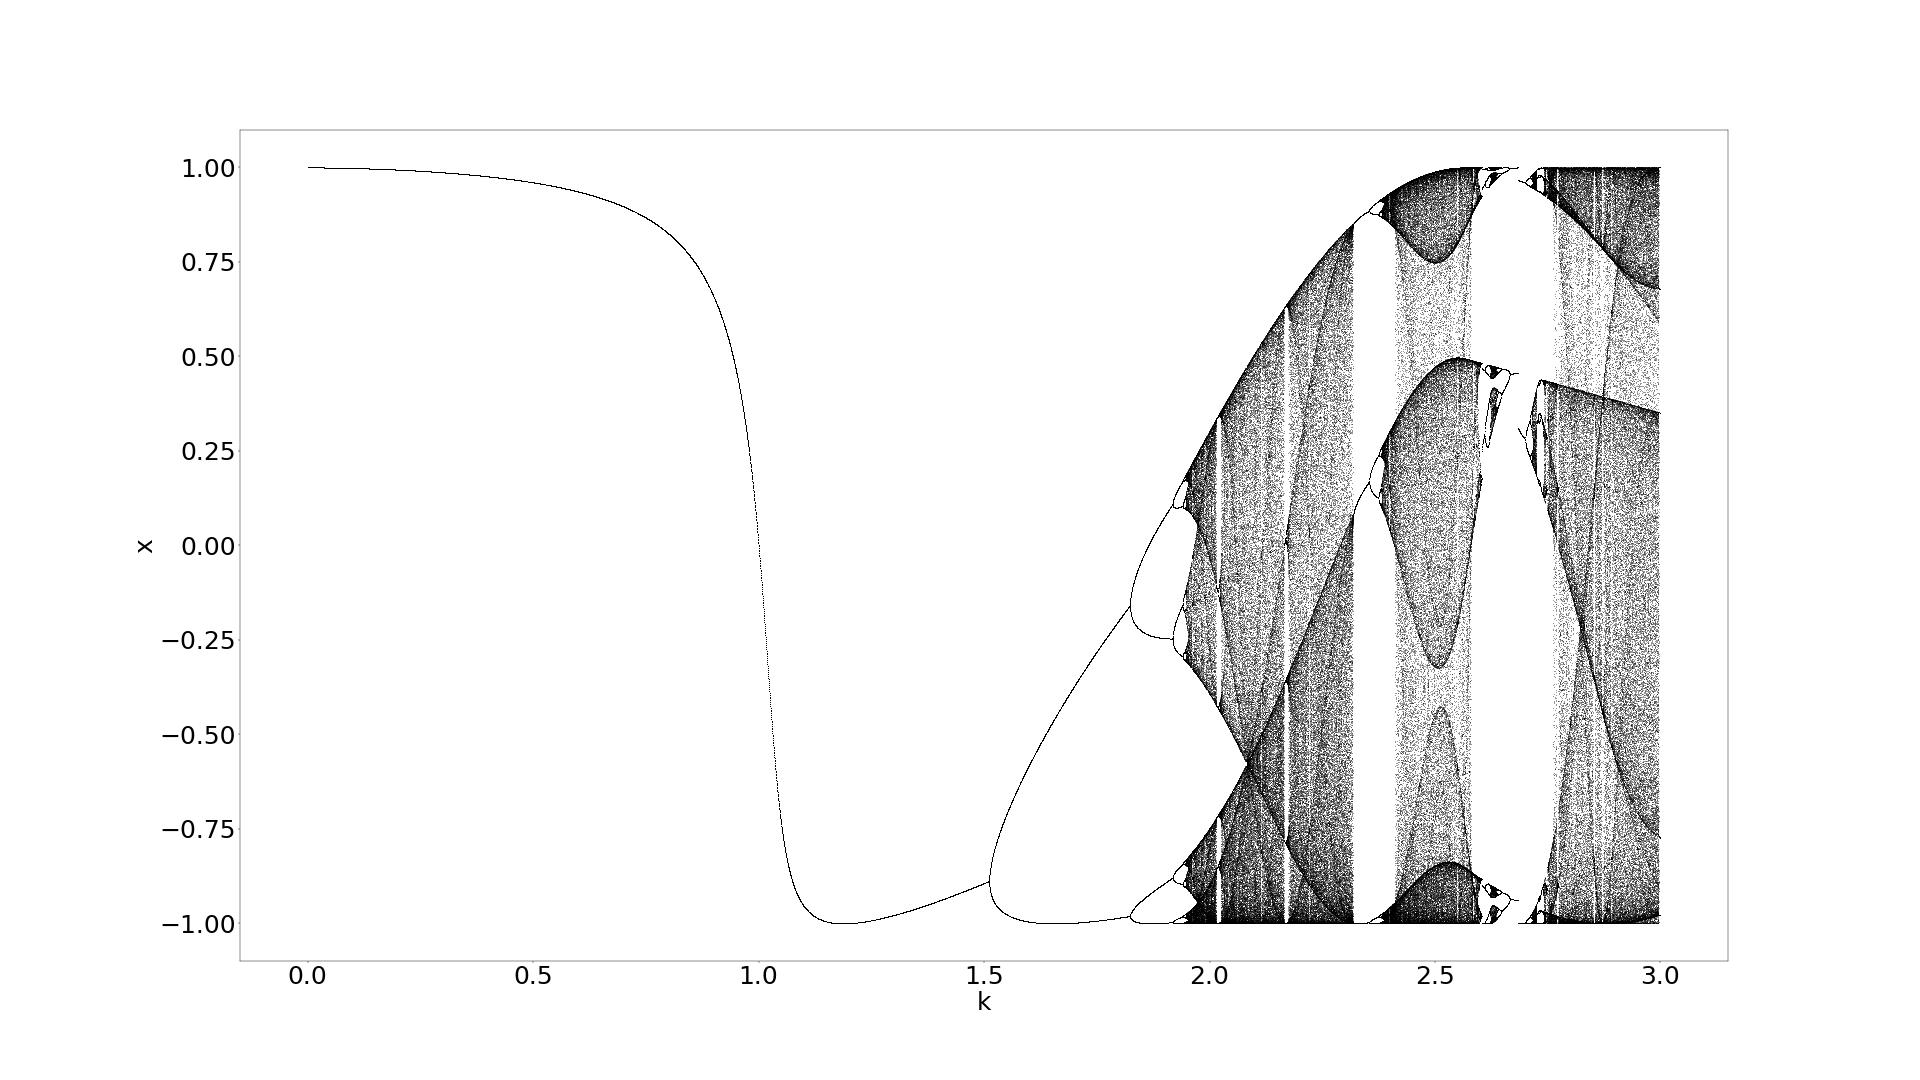
\includegraphics[width=1\linewidth]{LateX images/cheb q=0.9/g1}
	\caption{Διάγραμμα διακλάδωσης, για $q=0.9$.}
	\label{f:g65}
\end{figure}


\begin{figure}[ht]
	\centering
	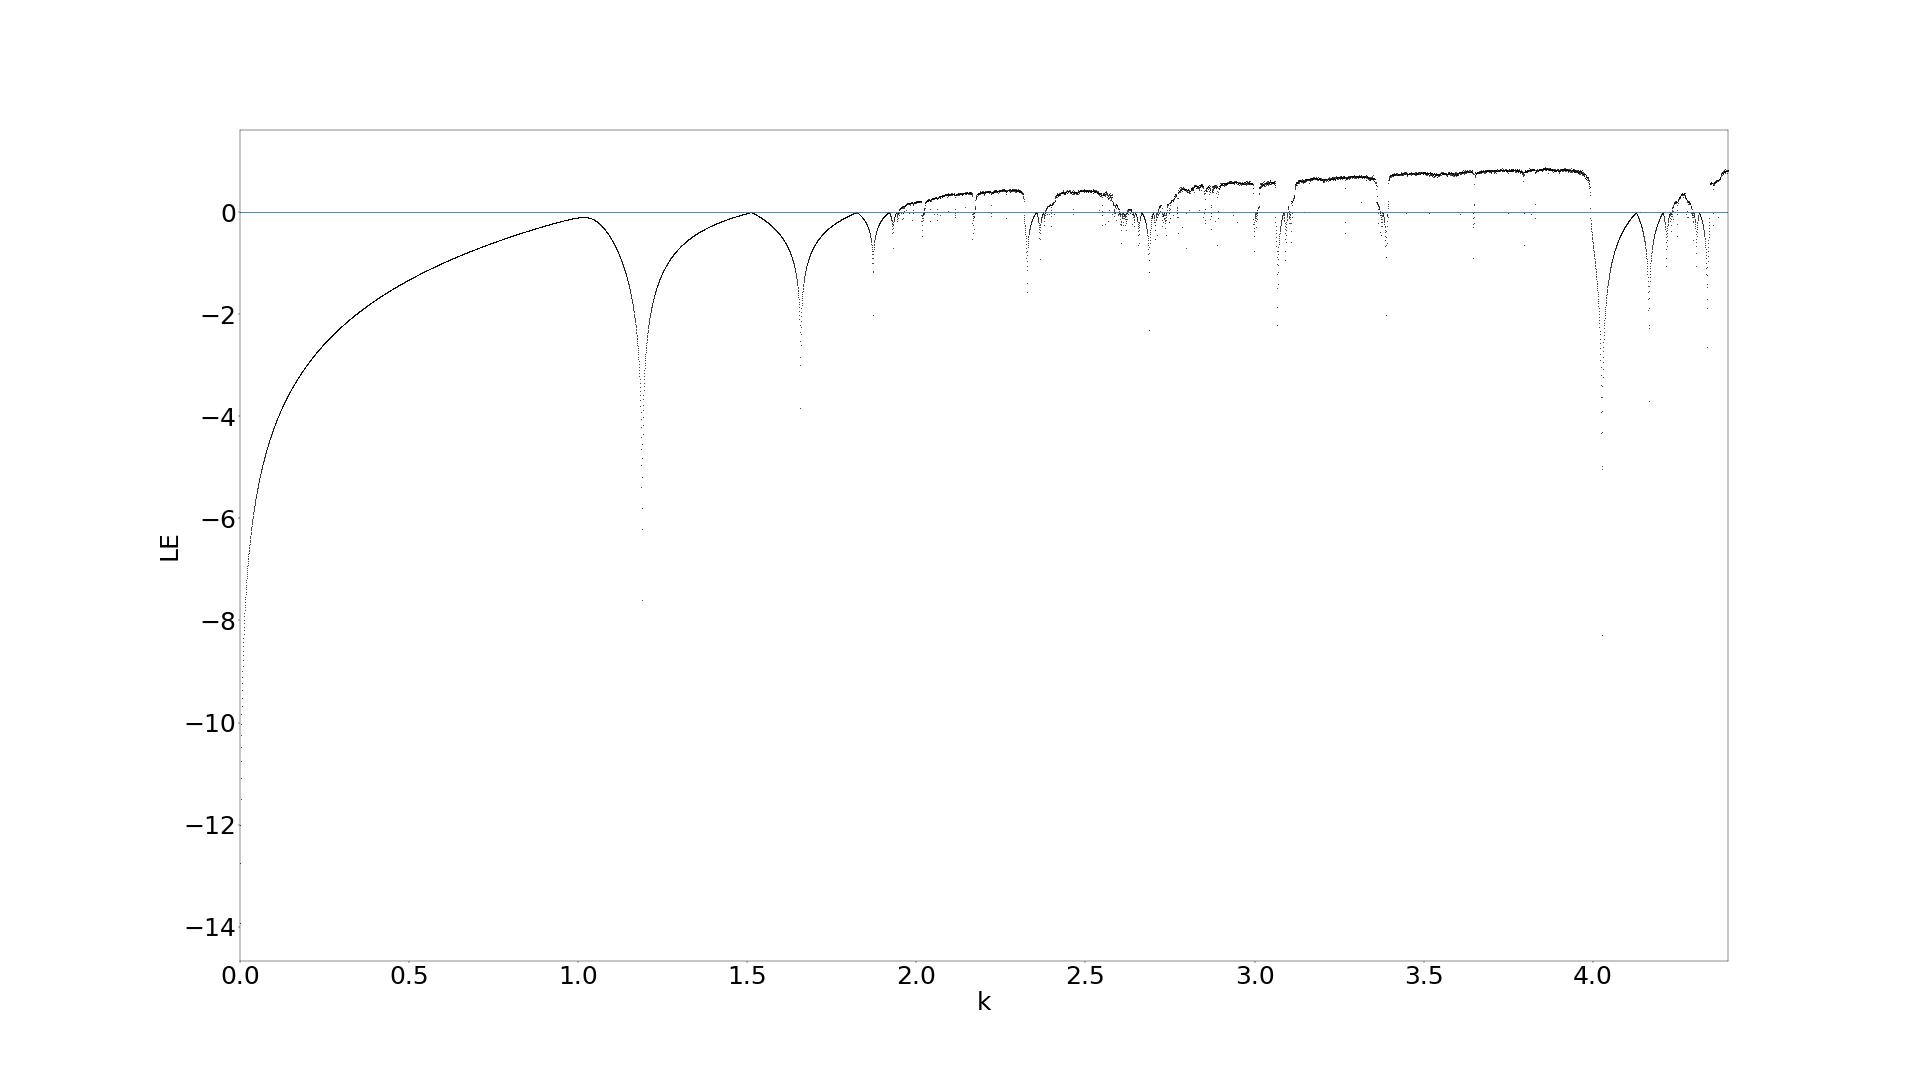
\includegraphics[width=1\linewidth]{LateX images/cheb q=0.9/g2}
	\caption{Διάγραμμα των εκθετών Lyapunov σε συνάρτηση με την παράμετρο k, για $q=0.9$.}
	\label{f:g66}
\end{figure}


\begin{figure}[ht]
	\centering
	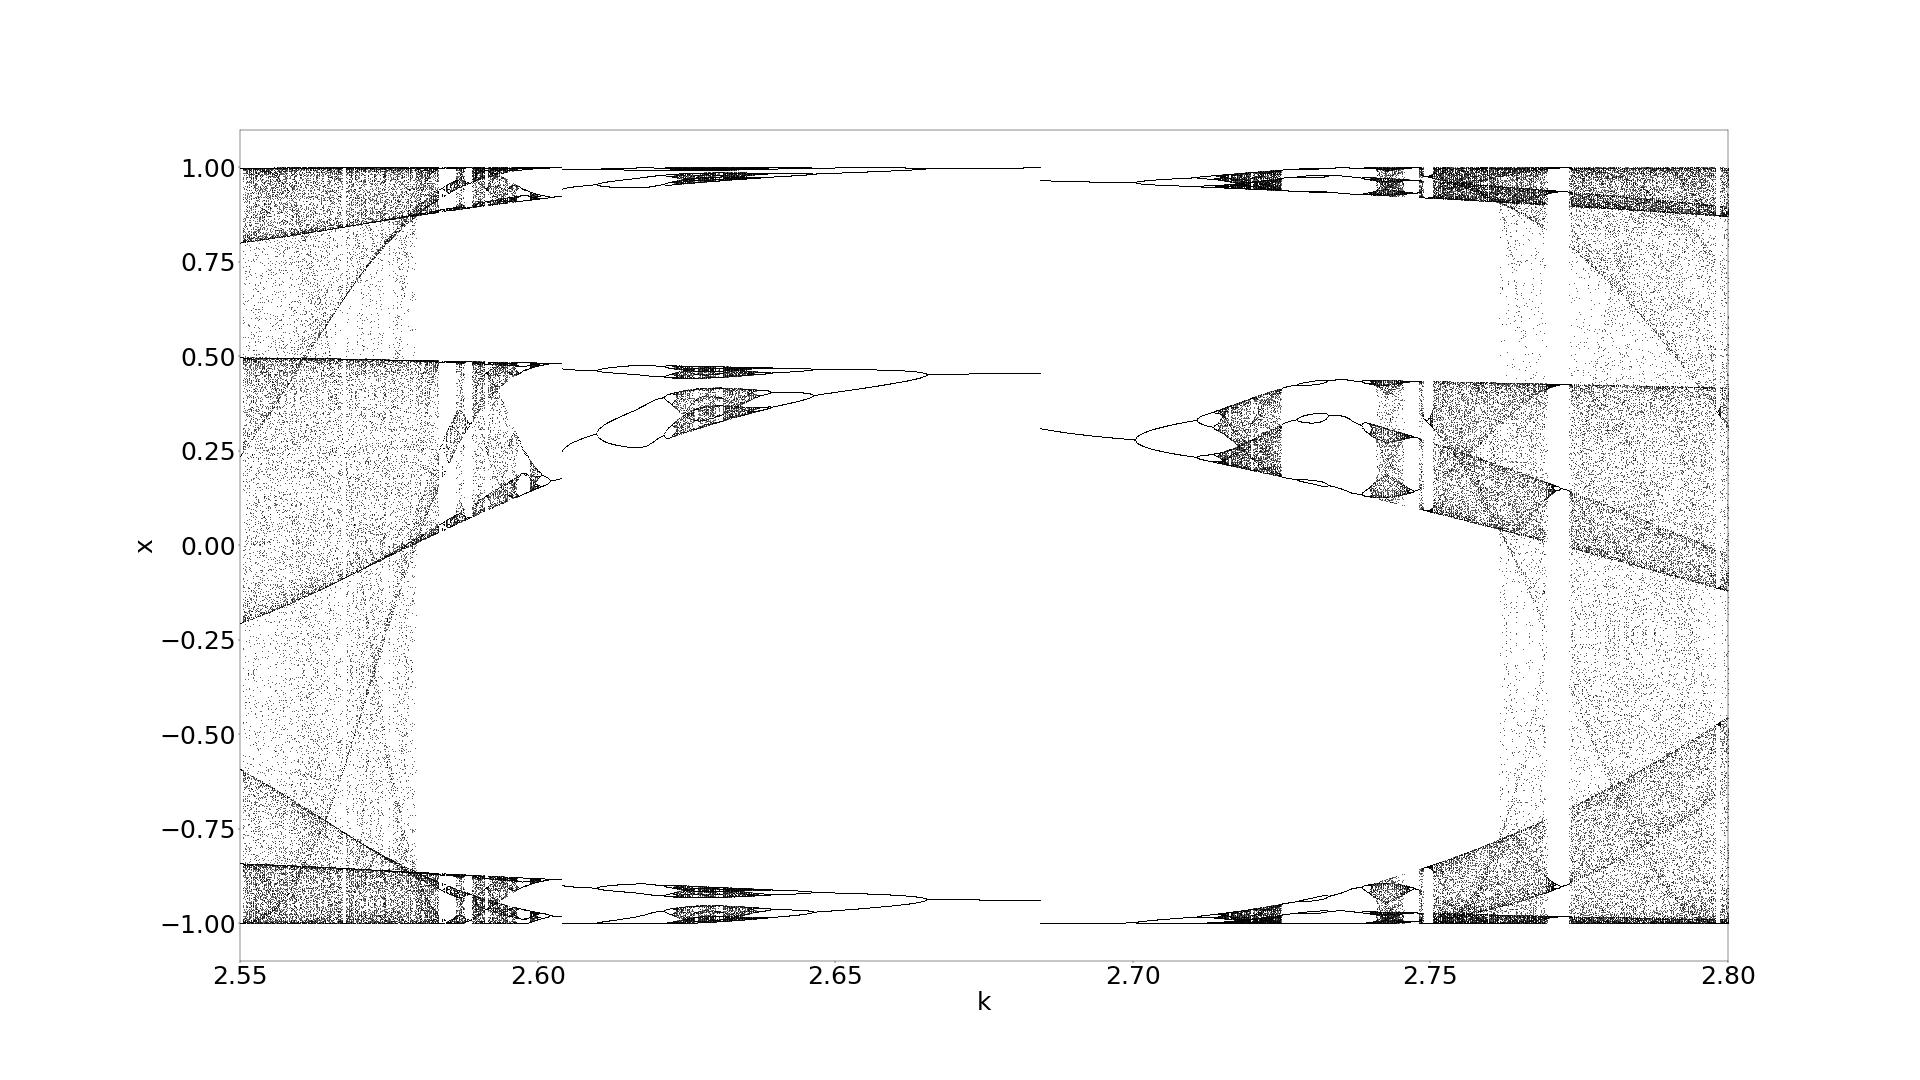
\includegraphics[width=\textwidth]{LateX images/cheb q=0.9/g3}
	\caption{Διάγραμμα διακλάδωσης για $2.55<k<2.8$. }
	\label{f:g67}
\end{figure}

\begin{figure}[ht]
	\centering
	\begin{subfigure}[b]{0.4\textwidth}
		\centering
		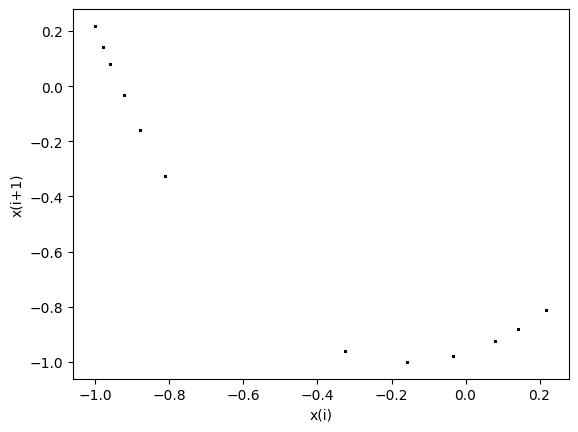
\includegraphics[width=\textwidth]{LateX images/cheb q=0.9/g4}
		\caption{Για $k=1.96$}
		\label{f:k142}
	\end{subfigure}
	\hfill
	\begin{subfigure}[b]{0.4\textwidth}
		\centering
		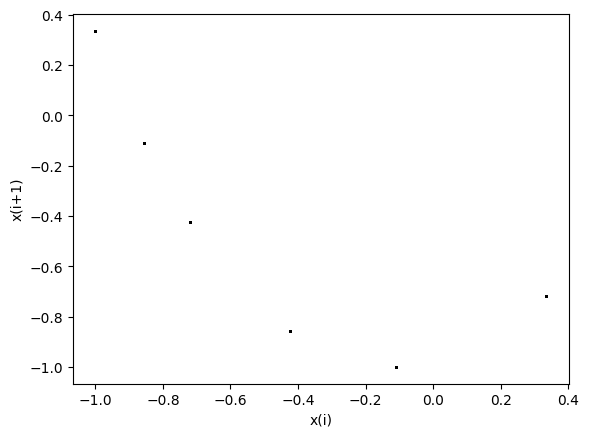
\includegraphics[width=\textwidth]{LateX images/cheb q=0.9/g5}
		\caption{Για $k=2.014$}
		\label{f:k143}
	\end{subfigure}
	\hfill
	\begin{subfigure}[b]{0.4\textwidth}
		\centering
		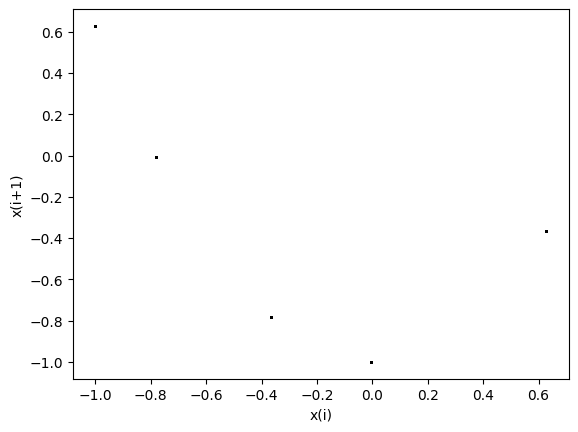
\includegraphics[width=\textwidth]{LateX images/cheb q=0.9/g6}
		\caption{Για $k=2.16$}
		\label{f:k144}
	\end{subfigure}
	\hfill
	\begin{subfigure}[b]{0.4\textwidth}
		\centering
		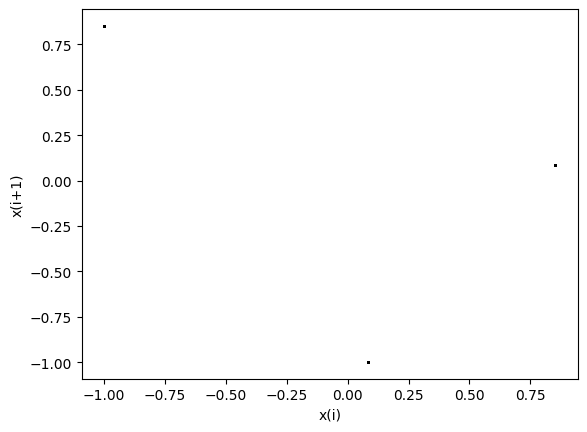
\includegraphics[width=\textwidth]{LateX images/cheb q=0.9/g7}
		\caption{Για $k=2.319$}
		\label{f:k145}
	\end{subfigure}
	\hfill
	\begin{subfigure}[b]{0.4\textwidth}
		\centering
		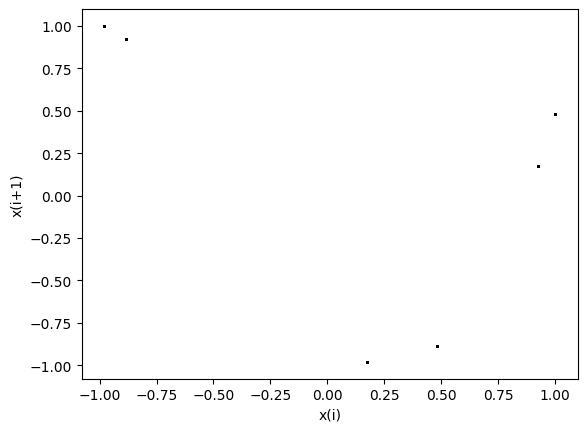
\includegraphics[width=\textwidth]{LateX images/cheb q=0.9/g8}
		\caption{Για $k=2.603$}
		\label{f:k146}
	\end{subfigure}
	\hfill
	\begin{subfigure}[b]{0.4\textwidth}
		\centering
		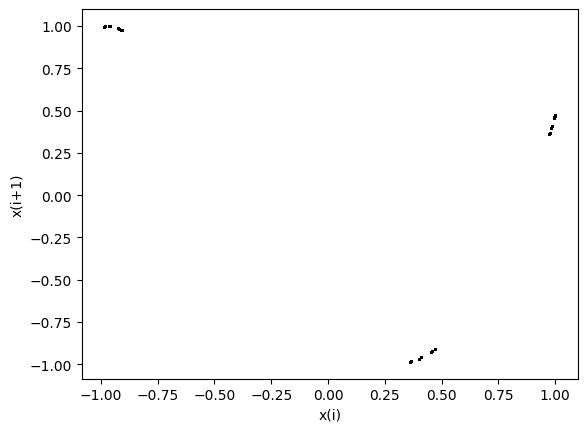
\includegraphics[width=\textwidth]{LateX images/cheb q=0.9/g9}
		\caption{Για $k=2.637$}
		\label{f:k147}
	\end{subfigure}
	\hfill	
	\begin{subfigure}[b]{0.4\textwidth}
		\centering
		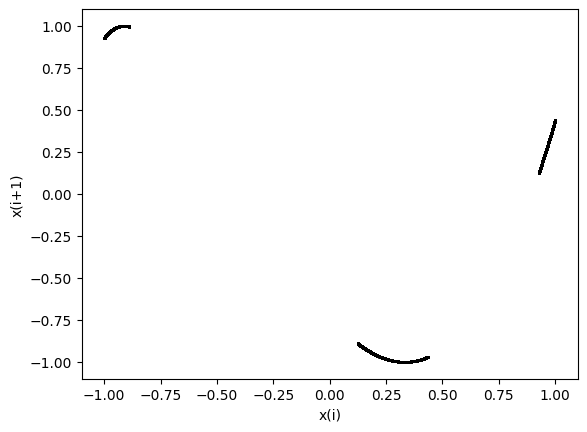
\includegraphics[width=\textwidth]{LateX images/cheb q=0.9/g10}
		\caption{Για $k=2.74$}
		\label{f:k148}
	\end{subfigure}
	\hfill	
	\begin{subfigure}[b]{0.4\textwidth}
		\centering
		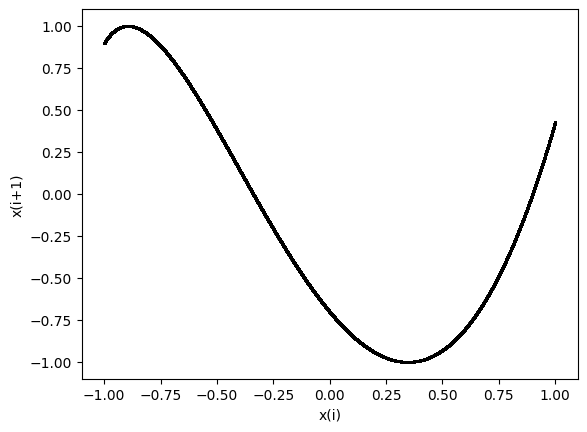
\includegraphics[width=\textwidth]{LateX images/cheb q=0.9/g11}
		\caption{Για $k=2.774$}
		\label{f:k149}
	\end{subfigure}
	\hfill
	
	\caption{Διαγράμματα της τιμής \(x_i\) σε συνάρτηση με την τιμή \(x_{i+1}\).}
	\label{f:k251}
\end{figure}

\clearpage

\section{Συμπεράσματα}

Σε αυτό το κεφάλαιο παρουσιάστηκε μία παραλλαγή του Χάρτη Chebysev, της οποίας βασικό χαρακτηριστικό είναι η χαοτική συμπεριφορά που διακρίνεται σε όλες τις περιπτώσεις που ελέχθηκαν για την παράμετρο q, όπως και για τα επι μερούς φαινόμενα που οδηγούν σε αυτήν.

Ειδικότερα, το συνηθέστερο φαινόμενο που παρατηρήθηκε σε όλες τις περιπτώσεις είναι αυτό της μετάβασης στο χάος μέσω του διπλασιασμού της περιόδου, ξεκινώντας απο διάστημα \emph{περιόδου-1}.
Για κάποιες παραμέτρους q εμφανίστηκε η ανάστροφη πορεία του συστήματος κατά την έξοδο του απο την χαοτική περιοχή, παρουσιάζοντας έτσι το φαινόμενο της αντιμονοτονικότητας (χαοτική φυσαλίδα).

Επίσης παρατηρήθηκε το φαινόμενο της υστέρησης δηλαδή "έσπαγε" η περιοδική συμπεριφορά, καθώς και το φαινόμενο των κρίσεων είτε εσωτερικών, είτε συνοριακών.

\newpage